\chapter{Исследовательская часть}

В данном разделе будут приведены примеры работы программы, а также проведен сравнительный анализ алгоритмов при различных ситуациях на основе полученных данных.

\section{Технические характеристики}

Технические характеристики устройства, на котором выполнялось тестирование представлены далее:
\begin{itemize}[label={---}]
	\item операционная система: Windows 11, x64;
	\item оперативная память: 8 Гб;
	\item процессор: AMD Ryzen 5 5500U с видеокартой Radeon Graphics 2.10~ГГц.
\end{itemize}

Во время замеров времени ноутбук был нагружен только встроенными приложениями окружения.

\section{Демонстрация работы программы}

На рисунках~\ref{img:run1}~--~\ref{img:run2} представлен результат работы программы.

\begin{figure}[H]
	\center{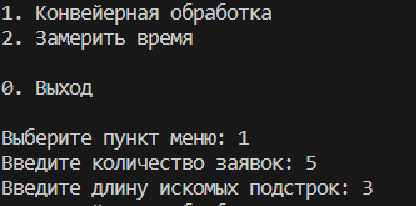
\includegraphics[scale=1.5]{img/run2}}
	\caption{Пример работы программы: вывод в консоль}
	\label{img:run1}
\end{figure}

\begin{figure}[H]
	\center{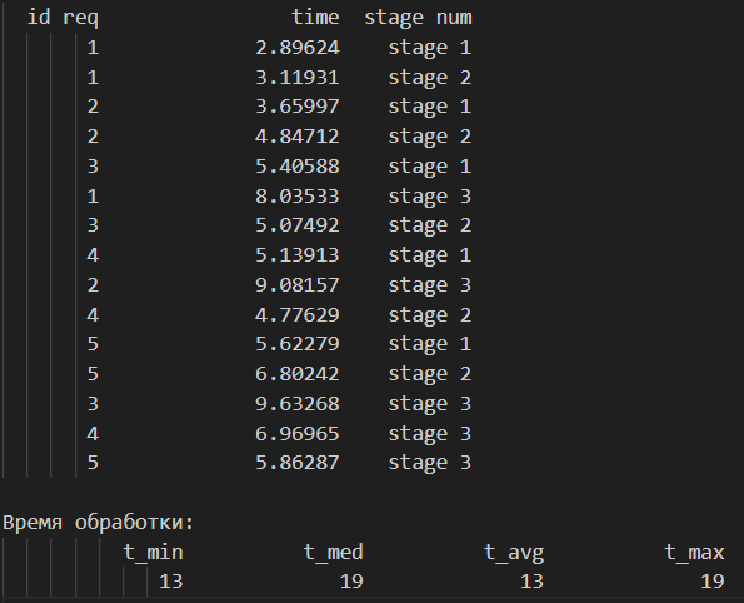
\includegraphics[scale=0.8]{img/run1}}
	\caption{Пример работы программы: вывод в лог-файл}
	\label{img:run2}
\end{figure}

\section{Время выполнения алгоритмов}

Как было сказано выше, используется функция замера процессорного времени $std::chrono::system\_clock::now()$. Функция возвращает пользовательское процессорное время типа \textit{float}.
Использовать функцию приходится дважды, затем из конечного времени нужно вычесть начальное, чтобы получить результат.

Замеры проводились для количества заявок от 100 до 1000 с шагом 100.

Результаты замеров приведены в таблице~\ref{tbl:time_mes} (время в мс).

\begin{table}[H]
	\begin{center}
		\begin{threeparttable}
			\captionsetup{justification=raggedright, singlelinecheck=off}
			\caption{Результаты замеров времени}
			\label{tbl:time_mes}
			\begin{tabular}{|r|r|}
				\hline
				Количество заявок & Время обработки всех заявок, мс\\
				\hline
				100 & 67.869 \\ \hline
				200 & 121.505  \\ \hline
				300 & 179.139  \\ \hline
				400 & 240.659  \\ \hline
				500 & 300.084  \\ \hline
				600 & 357.260  \\ \hline
				700 & 418.859  \\ \hline
				800 & 483.653  \\ \hline
				900 & 540.842  \\ \hline
				1000 & 585.003  \\ \hline
			\end{tabular}
		\end{threeparttable}
	\end{center}
\end{table}


На рисунке~\ref{img:graph} приведена визуализация результатов замеров.

\inputPdf{graph}{Визуализация результатов замеров}

\section{Вывод}

Как видно из графика \ref{img:graph}, время обработки растет линейно в зависимости от количества заявок. Так, например, при увеличении количества заявок в 10 раз, время увеличивается в 8,62 раза.